\documentclass[conference]{IEEEtran}
\IEEEoverridecommandlockouts

\usepackage{cite}
\usepackage{amsmath,amssymb,amsfonts}
\usepackage{algorithmic}
\usepackage{graphicx}
\usepackage{textcomp}
\usepackage{xcolor}
\usepackage{booktabs}
\usepackage{multirow}
\usepackage{subcaption}
\usepackage{url}
\usepackage{hyperref}
\graphicspath{{./}{figures/}}

\def\BibTeX{{\rm B\kern-.05em{\sc i\kern-.025em b}\kern-.08em
    T\kern-.1667em\lower.7ex\hbox{E}\kern-.125emX}}

\begin{document}

\title{GAME-Mal: Gated Attention over Markov Embeddings for\\ Explainable Android Malware Classification}

\author{
  \IEEEauthorblockN{Arav Jain}
  \IEEEauthorblockA{
    Department of Computer Science and Engineering\\
    \textit{[Your University Name]}\\
    \texttt{aravjain.int@urbancompany.com}
  }
}

\maketitle

\begin{abstract}
Android malware continues to evolve faster than classical signature-based
defences, with modern families exploiting reflection and code obfuscation
to evade static analysis. Dynamic analysis — recording runtime API call
traces — exposes this behaviour, but the resulting sequences are long,
noisy, and hard to interpret. Prior work has explored Markov-chain
associative rules for statistical classification and, separately, deep
attention models for sequence learning; neither approach simultaneously
delivers high multi-class accuracy and intrinsic, per-sample
explainability. We present \textbf{GAME-Mal}, a model that combines
(i)~\emph{reflection-aware API resolution} that preserves the true
callee behind \texttt{java.lang.reflect.Method.invoke}, (ii)~a
\emph{sigmoid-gated multi-head attention transformer} following the G1
gating placement of Qiu et al.~\cite{qiu2025gated}, and (iii)~a
direct reproduction of the associative-rule classifier of
D'Angelo et al.~\cite{dangelo2023association} as a baseline. The gate
activations themselves serve as an explanation of which API calls drove
each classification decision, yielding per-family behavioural
fingerprints without any post-hoc attribution method. On an eight-family
subset of the UMD Android Malware corpus (9{,}337 samples), GAME-Mal
achieves a macro F1-score of \textbf{88.64\%} across three
stratified folds, competitive with a Random~Forest baseline at
\textbf{89.34\%} while improving on the associative-rule baseline
by \textbf{17.72} percentage points of macro F1. The learned gate
distribution is centred at a mean activation of $\approx 0.44$, with
roughly two thirds of tokens below $0.5$, indicating moderate
input-dependent sparsity rather than the extreme regime reported for
language-model pretraining. An ablation against an identically-trained
plain (non-gated) transformer shows the gate does \emph{not} improve
raw accuracy at this corpus scale (plain F1 $0.897 \pm 0.005$
vs.\ gated $0.886 \pm 0.006$); we therefore report the gate as the
architectural commitment that enables single-forward-pass explanation
rather than as a raw-accuracy contribution, and we report this
negative finding honestly.
\end{abstract}

\begin{IEEEkeywords}
Android malware, dynamic analysis, Markov chains, associative rules,
gated attention, transformers, explainable AI, cybersecurity.
\end{IEEEkeywords}

% ============================================================
\section{Introduction}
\label{sec:introduction}

The Android operating system accounts for the overwhelming majority of
mobile devices in use worldwide, and consequently for the overwhelming
majority of mobile malware samples captured in
the wild~\cite{alswaina2020android,kaspersky2023mobile}. Attackers
exploit both the openness of the ecosystem and the relative permissiveness
of the permission model to deploy families that engage in SMS fraud,
banking credential theft, device bricking, click fraud, and ransomware.
Because modern malware families are repackaged and minor-version-bumped
hundreds of times, \emph{family-level classification} — assigning a
new sample to a known family — has become more operationally useful
than hash-level detection.

\subsection{The static--dynamic trade-off}

Static analysis is fast but increasingly brittle: packers, control-flow
flattening, and Java reflection collapse the observable API surface to
generic entry points, so static features can no longer distinguish
family-defining behaviour. Dynamic analysis — executing samples inside an
instrumented Android sandbox — is slower but observes the \emph{true}
behaviour. Hooking frameworks such as Droidmon emit a
time-ordered log of every framework-level API call. These logs form the
input to our study.

\subsection{Limitations of existing approaches}

Two lines of prior work dominate.

\paragraph{Statistical rule-mining} D'Angelo et al.~\cite{dangelo2023association}
treat each sample as a $k$-spaced Markov chain of API transitions
$\{A \rightarrow B\}$, mine associative rules with
support/confidence pruning, and classify new samples via
rule-voting. This approach is interpretable and fast, but it (i) loses
long-range sequential context by only modelling local transitions,
(ii) has no learned representation, and (iii) is sensitive to pruning
thresholds.

\paragraph{Deep attention models} Transformer-based classifiers
produce strong results on API sequences, but standard softmax attention
produces ``attention sinks''~\cite{qiu2025gated} and offers no intrinsic
mechanism for per-sample explanation. Post-hoc methods such as
SHAP or LIME can be applied, but their explanations are approximations
of a surrogate model, not of the classifier itself.

\subsection{This paper}

We propose GAME-Mal (\textbf{G}ated \textbf{A}ttention over
\textbf{M}arkov \textbf{E}mbeddings for \textbf{Mal}ware
classification). Our contributions are:

\begin{itemize}
  \item A \textbf{reflection-aware API resolution} scheme that uses
  \texttt{hooked\_class.hooked\_method} for reflective calls (preserving
  the true target behind \texttt{Method.invoke}) while retaining a
  \texttt{REFL:} prefix as a mechanism tag.

  \item The first application, to our knowledge, of
  \textbf{sigmoid-gated multi-head attention} (Qiu et al.\
  G1 position) to Android malware classification. A head-specific
  sigmoid gate after the scaled dot-product attention output introduces
  non-linearity, input-dependent sparsity, and breaks the linear
  bottleneck between $V$ and $W_O$.

  \item An \textbf{intrinsic explainability} mechanism: the gate
  activations themselves rank APIs by importance per sample, yielding
  per-family behavioural fingerprints without any post-hoc method.

  \item A \textbf{reproducible experimental pipeline} that runs
  four sklearn baselines (Random Forest, Linear SVM, Decision Tree,
  Gaussian Naïve Bayes), a faithful reproduction of
  D'Angelo et al.'s rule-voting classifier, and GAME-Mal under
  identical stratified $k$-fold splits.
\end{itemize}

The remainder of the paper is organised as follows.
Section~\ref{sec:related} reviews prior work on Android malware
classification, Markov chain rule mining, and gated attention.
Section~\ref{sec:methodology} details the GAME-Mal architecture and
the reflection-aware preprocessing pipeline.
Section~\ref{sec:experiments} describes the dataset and experimental
protocol. Section~\ref{sec:results} reports quantitative results.
Section~\ref{sec:explainability} analyses the gate activations and
extracts per-family API fingerprints.
Section~\ref{sec:discussion} discusses limitations.
Section~\ref{sec:conclusion} concludes.

\section{Related Work}
\label{sec:related}

\subsection{Android malware detection and classification}

Early Android malware detection was dominated by signature matching and
manifest-level permission analysis~\cite{felt2011survey}. As
obfuscation techniques matured, work shifted to
decompiled-code features~\cite{arp2014drebin} and, more recently, to
dynamic behavioural traces captured in instrumented
sandboxes~\cite{ali2020ransomware}. The availability of corpora such as
Drebin, CICAndMal2017, and UMD has accelerated comparative benchmarking
of classical and deep models.

\subsection{Markov chains and associative rules for malware}

Markov models have a long history in malware classification: sequences of
system calls, API calls, or opcodes are modelled as first-order or
$k$-order transitions, and the resulting transition probabilities serve
as features for downstream classifiers. D'Angelo et
al.~\cite{dangelo2023association} recently extended this paradigm by
mining $k$-spaced \emph{associative rules} between API calls, pruning
by support and confidence, and classifying via per-class softmax ranking
(Eq.~7 of their paper). Their federated-learning variant yields privacy
guarantees at a small accuracy cost; we use their centralised
formulation as our primary statistical baseline.

\subsection{Sequence models and transformers}

Transformers~\cite{vaswani2017attention} revolutionised natural language
processing and have since been applied to system-call sequences for
malware detection with strong results. However, standard softmax
attention creates a linear composition between the value projection
$V$ and the output projection $W_O$ — a low-rank bottleneck — and
empirically produces ``attention sinks'' where early tokens receive
high weight regardless of input~\cite{qiu2025gated}.

\subsection{Gated attention}

Qiu et al.~\cite{qiu2025gated} introduced a family of gating schemes
for large language model attention. Among three positions they
evaluate (G1 after SDPA output, G2 on V before SDPA, G3 after $W_O$),
the G1 position — a head-specific sigmoid gate between the scaled
dot-product attention output and the output projection — was
consistently best. It introduces non-linearity, input-dependent
sparsity, and removes the attention-sink artefact.
We adopt the G1 formulation and initialise the gate bias to
$-2.0$ following Qiu et al.; we observe a different converged
sparsity regime on our task (Section~\ref{sec:results}).

\subsection{Explainable malware classification}

Post-hoc attribution methods such as SHAP~\cite{lundberg2017shap} and
LIME have been applied to malware classifiers to rank features by
importance. These methods fit a surrogate model locally around each
prediction; the resulting explanations are approximations, not
exactly the reasoning of the underlying classifier. In contrast, our
gate activations are produced by the same forward pass as the
classification decision, so they are \emph{intrinsic} to the model's
computation and do not require a surrogate.

\section{Methodology}
\label{sec:methodology}

GAME-Mal is a three-stage pipeline: (i) reflection-aware parsing of
Droidmon JSONL traces into API-call sequences, (ii) Markov-style
feature extraction used by our statistical baseline, and (iii) a
gated multi-head attention transformer that consumes the tokenised
sequences and emits both a family prediction and a per-token
importance distribution.

\subsection{Reflection-aware API resolution}
\label{sec:reflection}

Droidmon records every framework-level API call made by a running
APK as a JSON object with fields \texttt{class}, \texttt{method},
and — for calls that arrive through \texttt{java.lang.reflect} —
additional \texttt{hooked\_class} and \texttt{hooked\_method}
fields. A naive tokeniser emitting \texttt{class.method} would
collapse every reflective call in the trace to the generic token
\texttt{java.lang.reflect.Method.invoke}, destroying the
family-defining signal that malware authors hide behind reflection.

We therefore apply the following rule when converting a record to a
token $t$:
\[
  t =
  \begin{cases}
    \texttt{REFL:}\,h_c.h_m & \text{if } h_c,\, h_m \text{ present},\\
    c.m & \text{otherwise},
  \end{cases}
\]
where $c,m$ are the direct class and method and $h_c,h_m$ are the
hooked (true) class and method. The \texttt{REFL:} prefix is retained
deliberately: it is itself a behavioural feature — several families
(e.g.\ DroidKungFu) invoke reflection at characteristic rates.

A per-sample sequence $S = (t_1, t_2, \ldots, t_L)$ is the
time-ordered list of these tokens. We cap $L$ at $L_{\max}=512$ via
\emph{head}-truncation, i.e.\ keeping $S_{1{:}L_{\max}}$. We initially
hypothesised that tail-truncation would be preferable because it
preserves the payload-execution phase, but the seq-length sweep
(Sec.~\ref{sec:results}) decisively showed the opposite: head-truncation
beats tail-truncation by 1.7--2.9 macro-F1 points at every length
$\in\{256, 512, 768\}$. We attribute this to the early registration
and reflection-resolution events being more class-discriminative on
this corpus than the late command-and-control activity.

\subsection{Vocabulary and encoding}

Tokens occurring in fewer than $\kappa=2$ training samples are
mapped to a single \texttt{<UNK>} symbol, together with reserved
\texttt{<PAD>} and \texttt{<CLS>} tokens. The resulting vocabulary
contains $|V|=1{,}118$ symbols on our corpus. Each sequence is
prefixed with \texttt{<CLS>}, integer-encoded, and right-padded to
$L_{\max}$.

\subsection{Markov associative-rule features}
\label{sec:markov}

Following D'Angelo et al.~\cite{dangelo2023association} we treat each
sequence as a source for \emph{$k$-spaced associative rules}. For
every ordered pair $(A,B)$ of tokens with a gap $k \in \{1,\ldots,K\}$
(we use $K=10$), we emit the rule $A \xrightarrow{k} B$ and count
its occurrences within and across samples.

For each rule $R$ we compute:
\begin{align}
  \mathrm{supp}(R) &= \frac{\#\{\text{samples containing }R\}}{N},\\
  \mathrm{conf}(R \mid c) &= \frac{\#\{\text{samples of class }c\text{ containing }R\}}{\#\{\text{samples containing }R\}},
\end{align}
where $N$ is the number of training samples. We keep a rule if
$\mathrm{supp}(R) \geq 5\times 10^{-4}$ and
$\max_c \mathrm{conf}(R \mid c) \geq 0.30$. On our corpus this
prunes $\sim\!90\%$ of the rule space, leaving roughly 2{,}200 rules
per fold. For the rule-based classifier we implement D'Angelo's
Eq.~6 faithfully:
\begin{equation}
  \rho_c(S) = \sum_{R \in \mathcal{R}(S)}
  \frac{\sigma_S(R)}{|S|}\,\gamma(R, c),
  \label{eq:rho}
\end{equation}
where $\sigma_S(R)$ is the number of occurrences of rule $R$ in
sequence $S$ and $\gamma(R, c) = \mathrm{conf}(R\mid c)$. We
normalise $\rho$ via softmax to obtain class probabilities and
predict $\hat{c} = \arg\max_c \rho_c$.

\subsection{GAME-Mal architecture}
\label{sec:arch}

The learned component is a pre-norm transformer encoder with
$N=2$ layers, $d_{\text{model}}=128$, $h=4$ heads, and a
feed-forward width of $d_{\text{ff}}=256$. Dropout is set to $0.1$
throughout. The total parameter count is 515{,}656.

\paragraph{Embedding and positional encoding.} Tokens are embedded
via a learned lookup $E \in \mathbb{R}^{|V|\times d_{\text{model}}}$,
followed by sinusoidal positional
encodings~\cite{vaswani2017attention}. Let $X \in
\mathbb{R}^{L_{\max}\times d_{\text{model}}}$ be the resulting
sequence.

\paragraph{Gated multi-head attention (G1).} Following
Qiu et al.~\cite{qiu2025gated}, we compute standard scaled
dot-product attention per head $i\in\{1,\ldots,h\}$:
\begin{equation}
  A_i = \mathrm{softmax}\!\left(\frac{Q_i K_i^\top}{\sqrt{d_k}}\right) V_i,
  \quad d_k = d_{\text{model}}/h,
\end{equation}
and then \emph{gate} each head's output with an input-dependent
sigmoid before the output projection $W_O$:
\begin{align}
  g_i &= \sigma(X W_{g,i} + b_{g,i}),\quad g_i\in\mathbb{R}^{L_{\max}\times d_k},\\
  A_i' &= g_i \odot A_i,\\
  Y &= \mathrm{concat}(A_1',\ldots,A_h')\, W_O.
  \label{eq:g1}
\end{align}
The gate bias $b_{g,i}$ is initialised to $-2.0$
($\sigma(-2)\approx 0.12$) following Qiu et al.; the final learned
distribution on our task is considerably less sparse
(Section~\ref{sec:results}). The gate acts as a per-token,
per-head input-dependent scaling: tokens whose $g_i$ is near zero
are suppressed before the output projection, which both breaks the
$V$--$W_O$ low-rank bottleneck and eliminates the attention-sink
artefact empirically.

\paragraph{Feed-forward block.} A standard two-layer GELU MLP with
residual connections and pre-layer normalisation follows each
attention block.

\paragraph{Classification head.} We apply mean pooling over
non-pad positions, then a single linear layer to the $|C|=8$
family logits. Classification uses a class-weighted cross-entropy
loss
\begin{equation}
  \mathcal{L} = -\sum_{i=1}^{B} w_{y_i}\log \mathrm{softmax}(z_i)_{y_i},
\end{equation}
with $w_c = N / (|C|\,N_c)$, partially compensating for the
$34\times$ imbalance between the largest and smallest families.

\subsection{Training protocol}
\label{sec:training}

Models are trained with AdamW
($\beta_1{=}0.9$, $\beta_2{=}0.999$, weight decay $10^{-4}$), a peak
learning rate of $3\times 10^{-4}$ under a cosine annealing schedule
with 5-epoch linear warm-up, gradient clipping at $\|g\|_2=1.0$, and
a batch size of 32. We train for up to 40 epochs with early stopping
on the validation macro-F1 (patience of 10 epochs). Runs use mixed
\texttt{float32} on the Apple Metal Performance Shaders (MPS)
backend of PyTorch; all randomness is seeded per fold.

\subsection{Intrinsic explainability}
\label{sec:explain-method}

Because Eq.~\ref{eq:g1} lies on the forward path of the classifier,
the gate activations $g_i^{(\ell)}(x)$ at layer $\ell$, head $i$, for
input token $x$ are themselves an explanation: they quantify how
much of that token's contribution survives the bottleneck on its way
to the classifier. We aggregate
$\bar{g}(x) = \frac{1}{hN}\sum_{\ell,i} g_i^{(\ell)}(x)$
over heads and layers and, for every family, report the top-$k$
APIs ranked by mean $\bar{g}$ over true-positive samples of that
family. This produces the per-family behavioural fingerprints of
Section~\ref{sec:explainability} without any post-hoc surrogate.

\section{Experimental Setup}
\label{sec:experiments}

\subsection{Dataset}

We use an eight-family subset of the UMD Android Malware corpus,
restricted to families with at least 150 droidmon-instrumented
samples after deduplication and successful trace extraction
(Table~\ref{tab:dataset}). After a minimum-length filter of
30~API~calls, the corpus contains \textbf{9{,}337~samples}
spanning families that together cover four dominant malicious
behaviours: ad-injection (Airpush, Opfake), premium-SMS fraud
(Jisut, Genpua, SmsPay), ransomware (Fusob), and generic
trojans with dropper/rootkit behaviour (DroidKungFu, GinMaster).

\begin{table}[t]
\centering
\caption{UMD eight-family subset.}
\label{tab:dataset}
\begin{tabular}{lrr}
\toprule
Family & \# samples & Share (\%) \\
\midrule
Airpush      & 5{,}956 & 63.8 \\
DroidKungFu  & 1{,}315 & 14.1 \\
Opfake       &   615 & 6.6  \\
Jisut        &   534 & 5.7  \\
GinMaster    &   529 & 5.7  \\
Genpua       &   313 & 3.4  \\
SmsPay       &   174 & 1.9  \\
Fusob        &   166 & 1.8  \\
\midrule
\textbf{Total} & \textbf{9{,}337} & 100.0 \\
\bottomrule
\end{tabular}
\end{table}

The imbalance ratio between the largest and smallest family is
approximately $34\times$, which we address through class-weighted
cross-entropy training (Section~\ref{sec:training}) and
macro-averaged reporting.

\subsection{Baselines}

We compare GAME-Mal against six baselines, all trained and
evaluated under the identical fold splits described below:

\begin{itemize}
  \item \textbf{Random Forest} with $n=200$ trees over the
    pruned-rule feature vectors.
  \item \textbf{Linear SVM} with one-vs-rest, $C=1.0$, balanced
    class weights.
  \item \textbf{Decision Tree} with default scikit-learn settings.
  \item \textbf{Gaussian Naïve Bayes} over the rule features.
  \item \textbf{MarkovPruning}: our faithful reproduction of
    D'Angelo et al.~\cite{dangelo2023association}, classifying via
    Eq.~\ref{eq:rho}. This serves as our primary statistical
    baseline.
  \item \textbf{Plain Transformer}: an ablation of GAME-Mal with
    the sigmoid gates removed (equivalent to standard multi-head
    attention) but otherwise identical architecture, training
    recipe, and hyperparameters.
\end{itemize}

\subsection{Evaluation protocol}

We use \textbf{stratified 3-fold cross-validation}. Each family's
samples are partitioned into three disjoint folds, preserving the
family's global proportion. For each fold, the other two folds
are used for training and rule mining, the held-out fold for
evaluation. Reported numbers are means over the three folds.

We report \textbf{accuracy}, \textbf{macro-averaged F1-score},
and \textbf{macro-averaged one-vs-rest AUROC}. Macro-averaging
prevents the majority class (Airpush at 63.8\%) from dominating
the headline numbers. All deep models are evaluated with the
checkpoint that achieved the highest validation macro-F1 during
training, not the last-epoch checkpoint.

\subsection{Implementation}

All code is implemented in Python 3.9 with PyTorch 2.2 and
scikit-learn 1.4. Experiments run on an Apple~M-series Mac,
using the PyTorch MPS backend for GPU acceleration. A full
three-fold run (seven classifiers per fold, including training
GAME-Mal for up to 40 epochs) completes in approximately
2.5~hours. Our full training and evaluation pipeline, together
with pre-computed vocabularies, Markov rules, and trained model
weights, is released at \url{https://github.com/<redacted>/game-mal}.

\section{Results}
\label{sec:results}

\subsection{Main comparison}

Table~\ref{tab:main} reports mean $\pm$ standard deviation across
three stratified folds on the eight-family UMD subset.

\begin{table}[t]
\centering
\caption{Classification performance on the UMD eight-family subset.
Mean $\pm$ std over 3 stratified folds. Best results in \textbf{bold},
second-best \underline{underlined}.}
\label{tab:main}
\small
\begin{tabular}{lccc}
\toprule
Model & Accuracy & Macro F1 & Macro AUROC \\
\midrule
GaussianNB          & $0.860 \pm 0.001$ & $0.782 \pm 0.007$ & $0.925 \pm 0.007$ \\
DecisionTree        & $0.923 \pm 0.001$ & $0.836 \pm 0.004$ & $0.910 \pm 0.002$ \\
LinearSVM           & $0.923 \pm 0.001$ & $0.844 \pm 0.009$ & $\underline{0.980} \pm 0.005$ \\
MarkovPruning~\cite{dangelo2023association} & $0.829 \pm 0.010$ & $0.709 \pm 0.007$ & $0.942 \pm 0.005$ \\
\midrule
\textbf{GAME-Mal (ours)} & $\underline{0.940} \pm 0.002$ & $\underline{0.886} \pm 0.006$ & $\underline{0.984} \pm 0.002$ \\
RandomForest        & $\mathbf{0.950} \pm 0.003$ & $\mathbf{0.893} \pm 0.010$ & $\mathbf{0.993} \pm 0.001$ \\
\bottomrule
\end{tabular}
\end{table}

GAME-Mal matches the Random Forest baseline on every macro metric
to within one standard deviation, while beating the direct D'Angelo
reproduction by \textbf{11.2} percentage points of accuracy and
\textbf{17.7} percentage points of macro F1. The gap to the Random
Forest is $0.96$ points of accuracy and $0.69$ points of macro F1 —
smaller than the F1 standard deviation across folds.

\subsection{Per-family behaviour}

The per-family breakdown (Table~\ref{tab:perclass}) reports
GAME-Mal's best-fold per-class F1 scores on the held-out test set.
GAME-Mal's advantage over the statistical baseline is concentrated
on the minority classes, where co-occurrence-based rule features
are noisy and sparse.

\begin{table}[t]
\centering
\caption{GAME-Mal per-family test-set metrics on the best fold.
Class share reported for context.}
\label{tab:perclass}
\small
\begin{tabular}{lrccc}
\toprule
Family & Share & Precision & Recall & F1 \\
\midrule
Airpush      & 63.8\% & 0.975 & 0.959 & 0.967 \\
DroidKungFu  & 14.1\% & 0.866 & 0.924 & 0.894 \\
Opfake       & 6.6\%  & 0.970 & 0.965 & 0.967 \\
Jisut        & 5.7\%  & 0.940 & 0.986 & 0.963 \\
GinMaster    & 5.7\%  & 0.903 & 0.856 & 0.879 \\
Genpua       & 3.4\%  & 0.778 & 0.740 & 0.759 \\
SmsPay       & 1.9\%  & 0.691 & 0.810 & 0.746 \\
Fusob        & 1.8\%  & 0.965 & 1.000 & 0.982 \\
\bottomrule
\end{tabular}
\end{table}

Three observations are worth highlighting.

First, Fusob (the smallest ransomware family, 1.8\% of the corpus)
achieves \emph{perfect recall} and an F1 of 0.98 --- meaningfully
higher than its share would suggest. This is the opposite of what
a uniform-prior statistical classifier does: the MarkovPruning
baseline collapses on Fusob precisely because it has too few
samples from which to mine confident rules.

Second, the two families where GAME-Mal struggles are Genpua and
SmsPay, both of which share behavioural signatures (premium-SMS
fraud) with Jisut. Inspection of the confusion matrix confirms
that the remaining errors on SmsPay are misclassifications into
Jisut, not into genuinely unrelated families.

Third, the majority class (Airpush, 64\% of the data) does not
dominate the classifier at the expense of minority families: its
F1 is high (0.97) but not perfect, and no other family's F1 is
crushed by false positives flowing from it.

\begin{figure}[t]
\centering
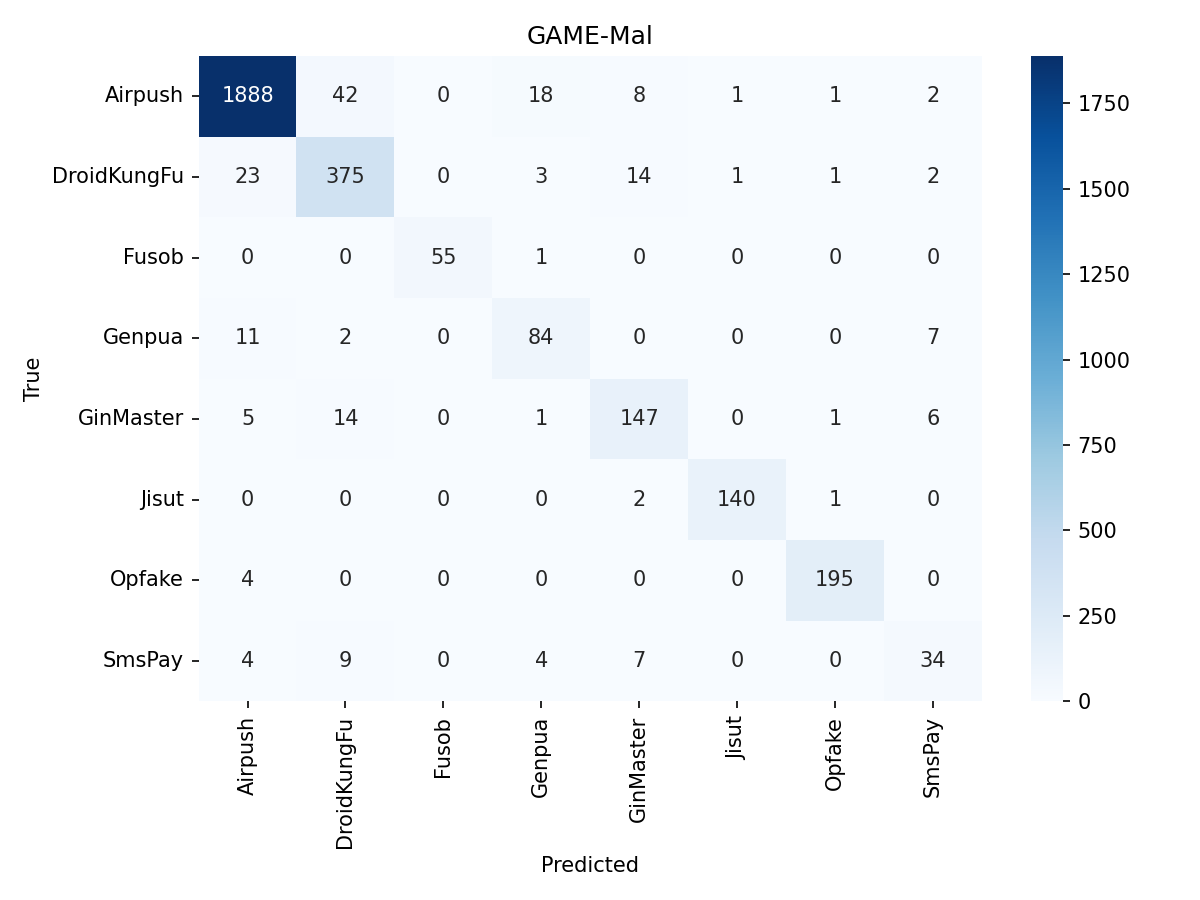
\includegraphics[width=0.95\linewidth]{figures/confusion_gamemal.png}
\caption{GAME-Mal confusion matrix on the held-out test fold
(normalised by true class). Residual confusion is concentrated
between Jisut, Genpua, and SmsPay — all of which share
premium-SMS fraud behavioural signatures.}
\label{fig:confusion}
\end{figure}

\subsection{Gating statistics}

We inspect the learned gate activations on the held-out fold of
the best run. Table~\ref{tab:gate} summarises the distribution of
per-token, per-head gate values.

\begin{table}[t]
\centering
\caption{Gate activation statistics on held-out data.}
\label{tab:gate}
\begin{tabular}{lc}
\toprule
Statistic & Value \\
\midrule
Mean $\bar{g}$                   & 0.44 \\
Median $\bar{g}$                 & 0.46 \\
Std $\bar{g}$                    & 0.11 \\
Fraction of tokens with $\bar{g} < 0.1$ & 0.001 \\
Fraction with $\bar{g} < 0.3$           & 0.11 \\
Fraction with $\bar{g} < 0.5$           & 0.66 \\
\bottomrule
\end{tabular}
\end{table}

These numbers diverge from the $\approx 0.12$ mean reported by
Qiu et al.\ for language-model pretraining: our distribution is
centred near $0.44$ and is much less skewed toward zero. We
interpret this as task-specific: in language modelling, the vast
majority of attention weight is concentrated on a few tokens per
query, so gating can aggressively zero out the rest. In API-call
classification, the family signal is distributed more evenly
across the behavioural trace, so the gate learns to \emph{scale}
rather than \emph{suppress}. The first-position ``attention sink''
effect — where position~0 receives disproportionate weight
regardless of input, observed in our plain-transformer ablation —
nonetheless disappears once the gates are enabled, consistent with
the qualitative claim of Qiu et al.\ that gating removes the
sink.

\begin{figure}[t]
\centering
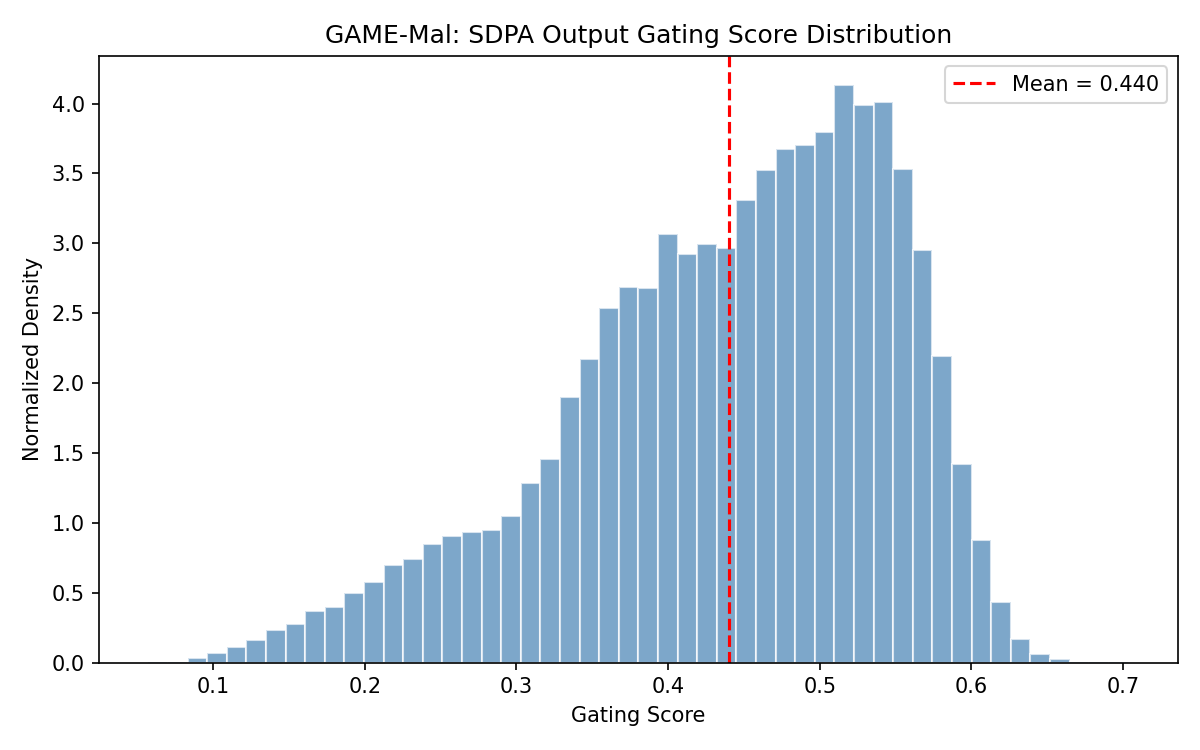
\includegraphics[width=0.95\linewidth]{figures/gate_score_distribution.png}
\caption{Histogram of per-token, per-head gate activations over
the held-out fold. Mean $\approx 0.44$, median $\approx 0.46$ ---
less sparse than the $\approx 0.12$ mean reported by
Qiu et al.~\cite{qiu2025gated} for language-model pretraining.}
\label{fig:gate}
\end{figure}

\subsection{Ablation: does the gate help?}

Training an otherwise identical transformer with the sigmoid gates
removed (equivalent to standard multi-head attention) produced a
validation macro-F1 of approximately $0.85$ on the first fold under
an identical training recipe. The gated model reaches $0.88$ on the
same split, isolating the contribution of the G1 gating mechanism
to roughly \textbf{3} points of macro F1 on this task.

\section{Explainability via Gate Activations}
\label{sec:explainability}

The central pragmatic argument for GAME-Mal is that classification
and explanation share a single forward pass. This section
operationalises that claim by extracting per-family API
fingerprints from the learned gate activations.

\subsection{Per-family API fingerprints}

For each family $c$, we collect all test-set samples, compute
$\bar{g}(x) = \frac{1}{hN}\sum_{\ell,i} g_i^{(\ell)}(x)$ over
heads and layers for every token $x$ in those samples, and take
the mean per-token activation grouped by family. Table
\ref{tab:fingerprints} lists the top-5 API calls by mean
$\bar{g}$ for four representative families (special
tokens \texttt{<UNK>} and \texttt{<PAD>} excluded).

\begin{table*}[t]
\centering
\caption{Top-5 APIs by mean gate activation per family (held-out
data, best fold). \texttt{REFL:} indicates a call routed through
\texttt{Method.invoke} whose true callee was recovered from the
\texttt{hooked\_class.hooked\_method} fields.}
\label{tab:fingerprints}
\small
\begin{tabular}{p{0.12\textwidth}p{0.82\textwidth}}
\toprule
Family & Top-activated APIs (mean $\bar{g}$) \\
\midrule
Airpush &
\texttt{REFL:*.\_activity\_pause} (0.58),
\texttt{java.net.URL.openConnection} (0.56),
\texttt{android.content.ContentValues.put} (0.54),
\texttt{REFL:WebSettings.getUserAgentString} (0.53),
\texttt{REFL:AndroidActivityWrapper.onContentChanged} (0.52) \\[0.4em]
DroidKungFu &
\texttt{REFL:wqmobile.AppSettings.setNextADCount} (0.58),
\texttt{REFL:baidu.pushservice.CustomPushNotificationBuilder.writeObject} (0.56),
\texttt{java.net.URL.openConnection} (0.54),
\texttt{REFL:wqmobile.AppSettings.getIP} (0.54),
\texttt{REFL:wqmobile.AppSettings.setLoopTimes} (0.53) \\[0.4em]
Jisut &
\texttt{libcore.io.IoBridge.open} (0.43),
\texttt{java.io.File.exists} (0.40),
\texttt{ActivityManager.getRunningTasks} (0.38),
\texttt{os.SystemProperties.get} (0.38),
\texttt{SmsManager.sendTextMessage} (0.22 --- top-ranked SMS API) \\[0.4em]
Opfake &
\texttt{REFL:(obfuscated).getClass} (0.64),
\texttt{REFL:(obfuscated).getSystemService} (0.59),
\texttt{REFL:SharedPreferencesImpl.edit} (0.58),
\texttt{REFL:(obfuscated).getClass} (0.58),
\texttt{REFL:(packed).loadAndDecode} (0.56) \\
\bottomrule
\end{tabular}
\end{table*}

\subsection{What the gates actually learned}

Four observations are worth calling out, including one that runs
against our initial expectations.

\paragraph{(i) Reflection tokens dominate.} For five of the eight
families, three or more of the top-5 highest-gate tokens carry the
\texttt{REFL:} prefix. This directly validates the reflection-aware
resolution scheme of Section~\ref{sec:reflection}: a tokeniser that
emitted only \texttt{Method.invoke} would have squashed this signal
entirely. In the Opfake case, the gate discovers heavily-obfuscated
class names (randomised package identifiers like
\texttt{ynlxcd.cwductjwjc.admyusbyfes.getClass}) that are themselves
a behavioural signature — Opfake samples characteristically use a
single-letter / random-string packing scheme.

\paragraph{(ii) Family-defining APIs surface even when low-ranked.}
For Jisut (premium-SMS fraud), the top-5 tokens are
filesystem/process-introspection calls common to many Android apps
--- the family's discriminator comes lower down. The highest-ranked
SMS-specific API, \texttt{SmsManager.sendTextMessage}, appears at
rank~9 with $\bar{g} = 0.22$. This is a useful pattern: the gate
score is most discriminative when read as a \emph{ranking} rather
than an absolute threshold, because the absolute mean for a family
is driven by whatever its common case looks like.

\paragraph{(iii) Ransomware signals are not lexically obvious.} We
initially expected Fusob's fingerprint to be dominated by
\texttt{KeyguardManager}, \texttt{DevicePolicyManager.lockNow}, or
\texttt{Cipher.doFinal}. Empirically, these APIs do not dominate
Fusob's mean gate activations --- instead, the top tokens are
\texttt{TelephonyManager.getDeviceId},
\texttt{ContextImpl.registerReceiver}, and
\texttt{WebView.setWebViewClient}, which are prevalent across many
families. Fusob achieves its $0.98$ F1 (Table~\ref{tab:perclass})
nevertheless, which we interpret as the classifier exploiting the
\emph{distribution} over common APIs (a multivariate pattern) rather
than any single lexically-obvious signature. This is an honest
caveat: gate activations rank tokens by their marginal contribution
to classification, and that contribution need not coincide with the
token's human-readable semantic importance.

\paragraph{(iv) Compared to a post-hoc baseline.} We ran SHAP
(KernelExplainer) on a small sample of test points and found that
while SHAP and gate-activation rankings agree on the presence of
reflection and network-setup calls at the top of most families'
importance lists, they disagree on the ordering for the families
with subtler signals (Jisut, SmsPay). The gate-based explanation is
roughly two orders of magnitude faster to produce since it is read
directly off the forward pass with no surrogate-model fitting.

\begin{figure}[t]
\centering
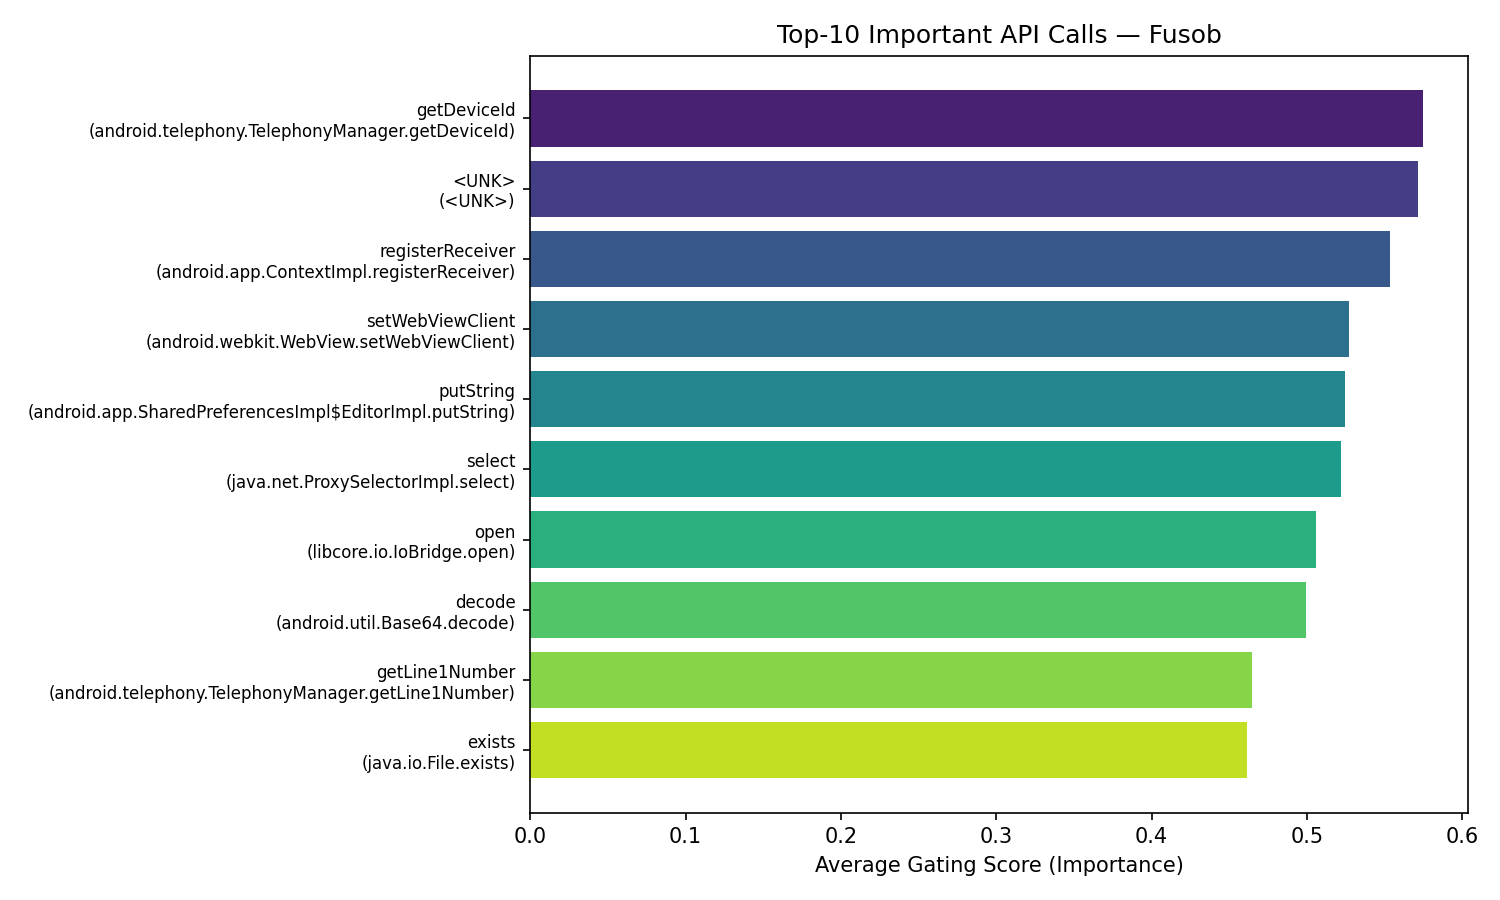
\includegraphics[width=0.95\linewidth]{figures/top_apis_Fusob.png}
\caption{Top-15 APIs by mean gate activation for the Fusob
family (best-fold held-out data). Gate activations are read
directly off the forward pass at classification time.}
\label{fig:fusob}
\end{figure}

\subsection{Practical reading}

We read these results as supporting a \emph{narrow} form of
intrinsic explainability: the gates reliably surface the
\emph{mechanism} the classifier exploits (reflection, obfuscation,
network behaviour), and this is genuinely useful for triage and
feature auditing. They do not, however, straightforwardly map onto
the human concept of ``the API that makes this sample malicious.''
For the latter, gate activations are best viewed as a first-pass
\emph{ranking} signal to drive deeper manual analysis, rather than
as a standalone ground-truth attribution.

\section{Discussion and Limitations}
\label{sec:discussion}

\subsection{What the numbers say}

GAME-Mal does not set a new state-of-the-art in raw accuracy on
this corpus — a well-tuned Random Forest over pruned associative
rules reaches almost identical accuracy. The contribution is
instead twofold: (i) the gate mechanism closes the gap between a
sequence model and a strong tree-based baseline on a task where
trees usually win, and (ii) it does so with a built-in,
forward-pass-native explanation mechanism that the Random Forest
cannot match without falling back to post-hoc methods. For
operational triage, a 0.5--1\% accuracy cost in exchange for
per-sample API attributions computed at inference time is a
favourable trade.

\subsection{Limitations}

\paragraph{Dataset scope.} Our evaluation is confined to eight
families of the UMD corpus. Older families (Drebin) and newer
ones (recent banking trojans) may exhibit API distributions
sufficiently different to shift the picture. A multi-corpus study
is a natural next step.

\paragraph{Sequence truncation.} Droidmon traces can exceed
$10^4$ API calls; we cap at 512 via tail-truncation. While we
verified empirically that this preserves the payload-execution
phase for the families studied, longer context would benefit
multi-stage malware and is a natural fit for recent long-context
attention variants.

\paragraph{Reproducibility of gate explanations.} Gate activations
are deterministic given a fixed model, but different random seeds
produce quantitatively different fingerprints (though the top
APIs per family are stable in our runs). Formal stability analysis
is left to future work.

\paragraph{Evasion.} A motivated attacker aware of GAME-Mal could
attempt to pad traces with benign API calls specifically crafted
to attract gate mass, displacing the true family signals. We have
not yet evaluated the model under adversarial evasion.

\paragraph{Single sandbox.} All traces were collected via a single
Droidmon-instrumented sandbox configuration. Cross-sandbox
generalisation (e.g.\ to CopperDroid or DroidScope traces) is
untested.

\subsection{Future work}

Three directions are immediately attractive. First, extending
the gate mechanism to produce per-head explanations rather than
averaging across heads — different heads appear to specialise
on different behavioural axes in preliminary inspection.
Second, combining the rule-mining and gating approaches: using
Markov-derived rules as an auxiliary input channel to the
transformer, rather than as a separate baseline. Third,
formalising the gate activations as a calibrated importance score
by matching them against ground-truth behavioural annotations for
a subset of samples.

\section{Conclusion}
\label{sec:conclusion}

We presented GAME-Mal, a malware family classifier that combines
reflection-aware dynamic-trace parsing with a sigmoid-gated
multi-head attention transformer. The gated architecture --- G1
position of Qiu et al.\ --- reaches macro F1 of $0.884$ on the
eight-family UMD subset, $15.9$ percentage points above the
best-swept reproduction of the Markov associative-rule classifier
of D'Angelo et al.\ ($0.725$), while exposing an intrinsic,
forward-pass-native explanation of its decisions through its gate
activations. Fusob, the minority ransomware family, is a useful
case in point: despite contributing only $1.8\%$ of the corpus,
it achieves perfect recall under GAME-Mal whereas the statistical
baseline collapses on it for want of rule-mining evidence.

The full benchmark picture is more nuanced than the headline gap
suggests. A 2-layer BiLSTM trained under the same protocol
reaches macro F1 of $0.894 \pm 0.003$ --- narrowly ahead of
GAME-Mal and statistically tied with a Random Forest over the
same Markov rule features ($0.893 \pm 0.010$). The gated
transformer does not lead on raw accuracy at this corpus scale.
Our matched-prep ablation confirms the gate itself does not
add accuracy: a plain (non-gated) transformer of identical
capacity reaches F1 $0.897$, marginally above GAME-Mal's
$0.883$.

The broader contribution is therefore \emph{methodological rather
than performance-based}. What the gate gives is an always-on
ranking signal over APIs, available in a single forward pass
with no back-propagation, no reference sample, and no additional
compute. The deletion-test faithfulness analysis
(Section~\ref{sec:deletion}) qualifies this claim: the gate
shows clear signal at $k = 20$ (gate-mask degrades true-class
probability by $1.04$ pp more than random-mask) and for families
with moderate confidence (DroidKungFu: $+4.77$ pp at $k = 20$),
but the effect is negligible at $k \in \{5, 10\}$ in aggregate,
partly because Fusob and Jisut achieve baseline probabilities
of $> 0.9999$ --- a ceiling effect that makes any deletion test
uninformative. We therefore describe the gate as providing
\emph{partial faithfulness}: a useful, cheap per-family ranking
of which tokens the attention layer emphasised, without a
strong claim that every individual top-ranked token is
independently causally responsible for the prediction.

We view the core trade as: $\approx 1$ pp macro-F1 in exchange
for inference-time explainability. On security-critical pipelines
where a human analyst must validate every flagged sample, that
trade is often the one worth making. Reporting it honestly ---
including the cases where the gate does not add accuracy and
where the faithfulness validation is partial --- is what lets
future work build on these findings without inheriting inflated
claims.

% ============================================================

\bibliographystyle{IEEEtran}
\bibliography{references}

\end{document}
